% !TeX program = lualatex
\documentclass[fleqn]{NotesClass}

\strictpagecheck

\usepackage{csquotes}
\usepackage{subcaption}

\usepackage[language=british]{biblatex}
\addbibresource{ref.bib}

\usepackage{tikz}
\usetikzlibrary{external}
\tikzexternalize[prefix=tikz-external/]

\usepackage{tikz-cd}
\AtBeginEnvironment{tikzcd}{\tikzexternaldisable}
\AtEndEnvironment{tikzcd}{\tikzexternalenable}

\usepackage[pdfauthor={Willoughby Seago},pdftitle={Notes from Algebraic Geometry Course},pdfkeywords={algebraic geometry},pdfsubject={Algebraic Geometry}]{hyperref}  % Should be loaded second last (cleveref last)
\colorlet{hyperrefcolor}{blue!60!black}
\hypersetup{colorlinks=true, linkcolor=hyperrefcolor, urlcolor=hyperrefcolor}
\usepackage[
capitalize,
nameinlink,
noabbrev
]{cleveref} % Should be loaded last

% My packages
\usepackage{NotesBoxes}
\usepackage{NotesMaths2}

\setmathfont[range={\int, \oint, \otimes, \oplus, \bigotimes, \bigoplus}]{Latin Modern Math}


% Highlight colour
\definecolor{my blue}{HTML}{084887}
\definecolor{my red}{HTML}{CA1551}
\definecolor{my green}{HTML}{17C3B2}
\definecolor{my yellow}{HTML}{F58A07}
\definecolor{my purple}{HTML}{CB9CF2}
\colorlet{highlight}{my green}

% Title page info
\title{Algebraic Geometry}
\author{Willoughby Seago}
\date{October 6th, 2025}
\subtitle{Notes from}
\subsubtitle{University of Glasgow}
\renewcommand{\abstracttext}{These are my notes from the SMSTC course \emph{Algebraic Geometry} taught by Dr Giulia Gugiatti and Prof Ivan Cheltsov. The lectures, and hence these notes, follow the \textit{Algebraic Geometry} notes of Andreas Gathmann. These notes were last updated at \printtime{} on \today{}.}

% Commands
% Maths
\newcommand{\subideal}{\trianglelefteq}
\newcommand{\affine}{\symbb{A}}
\newcommand{\ideal}[1]{\symfrak{#1}}
\newcommand{\isomorphic}{\cong}
\DeclareMathOperator{\Spec}{Spec}
\DeclareMathOperator{\codim}{codim}
\DeclareMathOperator{\Kdim}{Kdim}

\includeonly{appendices/comm-alg, appendices/topology}

\begin{document}
    \frontmatter
    \titlepage
    \innertitlepage{}
    \tableofcontents
    \listoffigures
    \mainmatter
    
    \chapter{Introduction}
    
    \section{Conventions and Notation}
    Throughout the notes the ground field, \(K\), will always be assumed to be \emph{algebraically closed}, up to the point where we introduce schemes.
    Taking \(K = \complex\) is usually reasonable.
    
    All rings, \(R\), are assumed to be \emph{commutative} with \emph{unity}.
    That \(J\) is an ideal of \(R\) will be denoted \(J \subideal R\).
    The ideal generated by a subset, \(S \subseteq R\), is denoted \(\langle S \rangle\).
    
    We write \(K[x_1, \dotsc, x_n]\) for the ring of polynomials with coefficients in \(K\) in the variables \(x_1, \dotsc, x_n\).
    We write \(f(a)\) to mean the evaluation of an element of this ring at the point \(a = (a_1, \dotsc, a_n) \in K^n\), and where no confusion may arise we'll usually call this point \(x = (x_1, \dotsc, x_n)\).
    
    The natural numbers, \(\naturals\), are assumed to contain \(0\).
    
    \section{Motivation}
    This section contains various motivating examples of algebro-geometric thinking, in varying levels of precision.
    Since the goal is to motivate some precision may be lacking.
    
    \subsection{Systems of Polynomial Equations}
    When we first learned algebra in high school it was to study the zeros of polynomials.
    Later we learned linear algebra, which it can be argued is the study of the zeros of systems of linear equations.
    Algebraic geometry combines these two fundamental fields into the study of zeros of systems of polynomials.
    
    Given \(f_1, \dotsc, f_m \in K[x_1, \dotsc, x_n]\) the basic object of study of algebraic geometry is the \defineindex{affine variety}
    \begin{equation}
        X = \{x \in K^n \mid f_i(x) = 0 \text{ for } i = 1, \dotsc, m\}.
    \end{equation}
    What questions can we ask about this set?
    Just as a single complex polynomial, \(f \in \complex[x]\), cannot be solved exactly for \(\deg f > 4\) we cannot possibly hope to explicitly list the points in \(X\).
    Instead we reason about the geometric structure of the solutions.
    We will ask geometric questions about \(X\), which we then aim to answer by an algebraic study of the \(f_i\).
    
    In the following sections we will give several examples of the sorts of geometric objects which can arise.
    We will focus on the existence of connections to other areas of mathematics.
    
    \subsection{Riemann Surfaces}
    Fix some positive integer, \(n\).
    We can define a curve\footnote{Note that this is a \enquote{curve} since it's complex dimension is \(1\) (we'll define dimension of affine varieties later, for now just use your intuition for the dimension of a manifold). Of course, in our pictures this single complex dimension is drawn as two real dimensions.}
    \begin{equation}
        c_n = \{(x, y) \in \complex^2 \mid y^2 = (x - 1)(x - 2)(x - 3) \dotsm (x - 2n)\} \subseteq \complex^2.
    \end{equation}
    We can view the defining equation as defining the quantity \(y\).
    Since we have \(y^2 = \dotso\) to find the value of \(y\) we have to take a square root.
    What we get depends on the value of \(x\).
    For most cases, specifically \(x \ne 1, 2, \dotsc, 2n\), we have
    \begin{equation}
        y = \pm \sqrt{(x - 1)(x - 2) \dotsm (x - 2n)}.
    \end{equation}
    For \(x = 1, 2, \dotsc, 2n\) we have
    \begin{equation}
        y = 0.
    \end{equation}
    Consider what values \(y\) can take.
    For \(x \ne 1, \dotsc, 2n\) we have two copies of \(\complex\), one for \(+ \sqrt{(x-1) \dotsm (x - 2n)}\) and one for \(-\sqrt{(x - 1) \dotsm (x - 2n)}\).
    For \(x = 1, \dotsc, 2n\) we only have one possible value, \(0\).
    The picture this suggests is two copies of \(\complex\) identified at the points \(1, \dotsc, 2n\).
    
    However, this isn't quite right.
    We know that \(z \in \complex^{\times}\) doesn't have a distinguished choice of \(\sqrt{z}\).
    Upon passing once around the origin they are exchanged.
    For example, if we take the path \(x = r\e^{i\theta}\), with \(r \ge 0\) fixed and \(\theta \in [0, 2\pi]\) then \(\sqrt{x} = \sqrt{r} \e^{i\theta/2}\).
    Then at \(\theta = 0\) we get \(\sqrt{r}\) and at \(\theta = 2\pi\) we get \(-\sqrt{r}\).
    The result is that as we go around the points \(x = 1, \dotsc, 2n\) we move from one copy of \(\complex\) to the other.
    
    Fortunately, we know how to deal with this, we take branch cuts between zeros.
    Take both copies of \(\complex\), and perform branch cuts along alternate intervals, \([1, 2], [3, 4], \dotsc, [2n - 1, 2n]\).
    For \(n = 3\) this produces \cref{fig:complex planes with branch cuts}.
    Now glue these along the cuts, which gives the picture \cref{fig:complex planes with branch cuts glued}.
    Finally, because it makes things nicer, add two points at infinity, one for each copy of \(\complex\), compactifying everything to get the picture \cref{fig:complex planes with branch cuts glued and compactified}.
    We see that this leaves us with a Riemann surface of genus \(g = n - 1\).
    This relates algebraic geometry to the theory of Riemann surfaces.
    
    \begin{figure}
        \centering
        \begin{subfigure}{0.8\textwidth}
            \centering
            \tikzsetnextfilename{riemann-surface-1}
            \begin{tikzpicture}
                \draw [very thick, rounded corners=1, my blue, fill=my blue!50] (0, -2) -- (8, -2) -- (9, 0) -- (1, 0) -- cycle;
                \draw [very thick, rounded corners=1, my blue, fill=my blue!50] (0, -0.5) -- (8, -0.5) -- (9, 1.5) -- (1, 1.5) -- cycle;
                
                \foreach \i in {1, 3, 5} {
                    \fill [white]  (1 + \i, 0.5) .. controls (1.3 + \i, 0.7) and (1.7 + \i, 0.7) .. (2 + \i, 0.5) .. controls (1.7 + \i, 0.3) and (1.3 + \i, 0.3) .. (1 + \i, 0.5);
                    \fill [white] (1 + \i, -1) .. controls (1.3 + \i, -0.8) and (1.7 + \i, -0.8) .. (2 + \i, -1) .. controls (1.7 + \i, -1.2) and (1.3 + \i, -1.2) .. (1 + \i, -1);
                    \draw [thick, my red] (1 + \i, 0.5) .. controls (1.3 + \i, 0.7) and (1.7 + \i, 0.7) .. (2 + \i, 0.5);
                    \draw [thick, my red] (1 + \i, 0.5) .. controls (1.3 + \i, 0.3) and (1.7 + \i, 0.3) .. (2 + \i, 0.5);
                    \draw [thick, my red] (1 + \i, -1) .. controls (1.3 + \i, -0.8) and (1.7 + \i, -0.8) .. (2 + \i, -1);
                    \draw [thick, my red] (1 + \i, -1) .. controls (1.3 + \i, -1.2) and (1.7 + \i, -1.2) .. (2 + \i, -1);
                }
                \foreach \i in {1, 2, 3, 4, 5, 6} {
                    \fill [my red] (1 + \i, 0.5) circle [radius=0.05];
                    \fill [my red] (1 + \i, -1) circle [radius=0.05];
                }
            \end{tikzpicture}
            \caption{Branch cuts along alternate intervals.}
            \label{fig:complex planes with branch cuts}
        \end{subfigure}
        
        \begin{subfigure}{0.8\textwidth}
            \centering
            \tikzsetnextfilename{riemann-surface-2}
            \begin{tikzpicture}
                \fill [my blue!50] (0, 0) arc (180:270:1) arc (90:0:1) arc (360:270:1) arc (90:180:1) -- ++ (10, 0) arc (0:90:1) arc (270:180:1) arc (180:90:1) arc (270:360:1) -- cycle;
                \draw [very thick, my blue] (0, 0) arc (180:270:1) arc (90:0:1) arc (360:270:1) arc (90:180:1);
                \draw [very thick, my blue] (10, -4) arc (0:90:1) arc (270:180:1) arc (180:90:1) arc (270:360:1);
                \draw [very thick, my blue, fill=white] (3.75, -2) circle [x radius = 0.5, y radius = 0.75];
                \draw [very thick, my blue, fill=white] (6.25, -2) circle [x radius = 0.5, y radius = 0.75];
                \draw [my red, very thick] (2, -2) .. controls (2.4, -2.2) and (2.85, -2.2) .. (3.25, -2);
                \draw [my red, very thick] (4.25, -2) .. controls (4.8, -2.2) and (5.2, -2.2) .. (5.75, -2);
                \draw [my red, very thick] (6.75, -2) .. controls (7.15, -2.2) and (7.6, -2.2) .. (8, -2);
                \draw [my red, very thick, dashed] (2, -2) .. controls (2.4, -1.8) and (2.85, -1.8) .. (3.25, -2);
                \draw [my red, very thick, dashed] (4.25, -2) .. controls (4.8, -1.8) and (5.2, -1.8) .. (5.75, -2);
                \draw [my red, very thick, dashed] (6.75, -2) .. controls (7.15, -1.8) and (7.6, -1.8) .. (8, -2);
            \end{tikzpicture}
            \caption{Gluing along branch cuts.}
            \label{fig:complex planes with branch cuts glued}
        \end{subfigure}
        
        \begin{subfigure}{0.8\textwidth}
            \centering
            \tikzsetnextfilename{riemann-surface-3}
            \begin{tikzpicture}
                \draw [very thick, my blue, fill=my blue!50] (0.5, 0.5) arc (90:180:0.5) arc (180:270:1) arc (90:0:1) arc (360:270:1) arc (90:180:1) arc (180:270:0.5) -- ++ (9, 0) arc (270:360:0.5) arc (0:90:1) arc (270:180:1) arc (180:90:1) arc (270:360:1) arc (0:90:0.5) -- cycle;
                \draw [very thick, my blue, fill=white] (3.75, -2) circle [x radius = 0.5, y radius = 0.75];
                \draw [very thick, my blue, fill=white] (6.25, -2) circle [x radius = 0.5, y radius = 0.75];
            \end{tikzpicture}
            \caption{Compactification by adding a point at infinity for each plane.}
            \label{fig:complex planes with branch cuts glued and compactified}
        \end{subfigure}
        \caption{Producing a Riemann surface from a curve}
    \end{figure}
    
    We can change our curve to
    \begin{equation}
        \{(x, y) \in \complex^2 \mid y^2 = (x - 1)^2(x - 2)(x - 3) \dotsm (x - 2n)\} \subseteq \complex^2.
    \end{equation}
    Then the same analysis can be applied, except that we have a singular point at the repeated root, \(x = 1\).
    This relates algebraic geometry to singularity theory.
    
    \subsection{Lines on Spaces}
    Consider the surface
    \begin{equation}
        X = \{(x_1, x_2, x_3) \in \reals^3 \mid 1 + x_1^3 + x_2^3 + x_3^3 - (1 + x_1 + x_2 + x_3)\} \subseteq \reals^3.
    \end{equation}
    This is called the \defineindex{Clebsch surface}.
    It's plotted in \cref{fig:clebsch surface}.
    This is a cubic surface because it's defined by a single cubic equation.
    It's possible to draw straight lines on this surface.
    One can ask how many such straight lines exist.
    The answer over \(\complex\), surprisingly, is always 27, at least under some mild conditions.
    The Clebsch surface has the nice property that all of these lines are real.
    Cubic surfaces are actually a weird middle ground, between the infinite families of lines on a quadratic surface, and the general absence of lines on surfaces defined by any higher degree equation.
    
    \begin{figure}
        \centering
        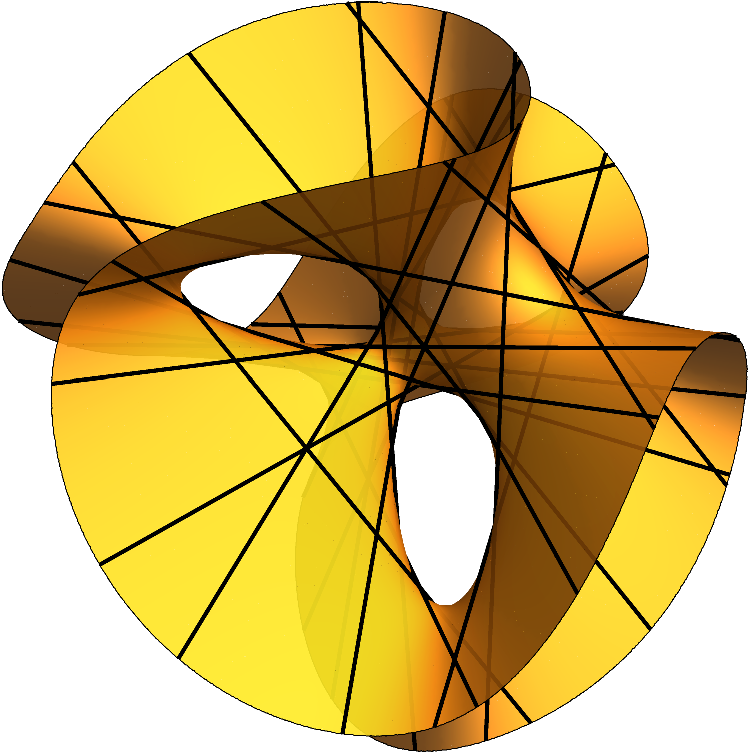
\includegraphics[width=0.8\textwidth]{images/clebsch-surface}
        \caption{The Clebsch surface, as well as the 27 lines which lie on it.}
    \end{figure}
    
    The question of how many geometric objects of a certain type exist is one of enumerative geometry, which makes heavy use of algebraic geometry.
    
    \subsection{String Theory}
    Strings, world sheets, those are surfaces, physicists should care about algebraic geometry.
    
    \subsection{Curves in Space}
    Consider the following curve
    \begin{equation}
        X = \{(x_1, x_2, x_3) = (t^3, t^4, t^5) \mid t \in \complex\} \subseteq \complex^3.
    \end{equation}
    This is a parametric definition of this surface.
    We can equally define it explicitly as
    \begin{equation}
        X = \{(x_1, x_2, x_3) \mid x_1^3 = x_2x_3, x_2^2 = x_1x_3, x_3^2 = x_1^2x_2\} \subseteq \complex^3.
    \end{equation}
    This is a surface, so it's two (complex) dimensional.
    However, we need all three of these equations to define it, if we remove any of them we don't get the same surface.
    This is very different to the world of linear algebra, where we'd have linear defining relations.
    There any codimension \(d\) subspace can be defined by \(d\) (linear) equations.
    Here \(X\) is one-dimensional, so it has codimension \(2\), but we need three equations to define it.
    
    The general problem of taking an affine variety, \(X\), defined as the vanishing set of some polynomials, and determining its dimension is actually very hard.
    We can use Gr\"obner bases to do this, but the algebra is pretty unwieldy, and we're forced to use computers to solve it most of the time.
    A Gr\"obner basis is a certain generating set of the ideal generated by the polynomials defining the affine variety.
    Actually, even defining dimension for an arbitrary affine variety is not that straight forward, but for now the intuition from manifolds and vector spaces should be enough.
    
    \subsection{Different Fields}
    Over \(\reals\) or \(\complex\) we can use real or complex analytic methods to study the zeros of polynomials, and hence affine varieties.
    
    Over \(\rationals\) or finite fields we can use number theoretic techniques to study the zeros of polynomials, and hence affine varieties.
    
    For example, Fermat's last theorem can be stated as the study of the affine variety
    \begin{equation}
        X = \{(x_1, x_2, x_3) \in \rationals^3 \mid x_1^n + x_2^n = x_3^n\},
    \end{equation}
    where the question we ask is if this has any non-trivial points.
    
    \chapter{Affine Varieties}
    \section{Affine Varieties}
    \begin{dfn}{Affine Space}{}
        \define{Affine \(\symbb{n}\)-space}\index{affine n-space@affine \(n\)-space} over \(K\) is the set
        \begin{equation}
            \affine^n = \affine_K^n \coloneq \{(a_1, \dotsc, a_n) \mid a_i \in K \forall i = 1, \dotsc, n\}.
        \end{equation}
    \end{dfn}
    
    Note that as sets \(\affine^n = K^n\).
    However, we write \(\affine^n\) when we wish to forget the additional algebraic structure of \(K^n\), specifically the vector space and ring, that is, we want to forget about the ability to scale, add and multiply elements.
    
    For the time being we will take \(\affine^n\) as our ambient space.
    Then a polynomial, \(f \in K[x_1, \dotsc, x_n]\), defines a \defineindex{polynomial function}
    \begin{align}
        \affine^n &\to K\\
        a &\mapsto f(a).
    \end{align}
    We'll usually call this function \(f\) as well.
    
    \begin{dfn}{Affine Variety}{}
        Let \(S \subseteq K[x_1, \dotsc, x_n]\) be some set of polynomials.
        The \defineindex{zero locus} or \defineindex{vanishing set} of \(S\), denoted \(V(S)\), is all points of \(\affine^n\) on which the polynomial functions defined by polynomials in \(S\) vanish.
        That is,
        \begin{equation}
            V(S) \coloneq \{x \in \affine^n \mid f(x) = 0 \forall f \in S\} \subseteq \affine^n
        \end{equation}
        Any subset of \(\affine^n\) of this form is called an \defineindex{affine variety}.
    \end{dfn}
    
    \begin{wrn}
        Note that some authors require that affine varieties have the additional property of being irreducible.
        These authors would then call all sets like \(V(S)\) \define{affine algebraic sets}\index{affine algebraic set}.
    \end{wrn}
    
    \begin{ntn}{}{}
        If \(S = \{f_1, \dotsc, f_n\}\) is a finite set we write
        \begin{equation}
            V(S) = V(\{f_1, \dotsc, f_n\}) = V(f_1, \dotsc, f_n).
        \end{equation}
    \end{ntn}
    
    There are some properties we can immediately prove about affine varieties.
    
    \begin{lma}{Reversal of Inclusion}{lma:V reverses inclusion}
        If \(S_1 \subseteq S_2 \subseteq K[x_1, \dotsc, x_n]\) then \(V(S_2) \subseteq V(S_1)\).
        \begin{proof}
            Suppose \(x \in V(S_2)\).
            Then \(f(x) = 0\) for all \(f \in S_2\), and so certainly \(f(x) = 0\) for \(f \in S_1 \subseteq S_2\), and thus \(x \in V(S_1)\).
        \end{proof}
    \end{lma}
    
    \begin{lma}{Union}{lma:union of defining equations}
        If \(S_1, S_2 \subseteq K[x_1, \dotsc, x_n]\) then \(V(S_1) \cup V(S_2) = V(S_1 S_2)\) where
        \begin{equation}
            S_1 S_2 = \{fg \mid f \in S_1, g \in S_2\}.
        \end{equation}
        \begin{proof}
            We start by showing that \(V(S_1) \cup V(S_2) \subseteq V(S_1 S_2)\).
            Suppose that \(x \in V(S_1) \cup V(S_2)\).
            Then \(x \in V(S_1)\), so \(f(x) = 0\) for all \(f \in S_1\), and \(x \in V(S_2)\), so \(g(x) = 0\) for all \(g \in S_2\).
            Thus, for \(f \in S_1\) and \(g \in S_2\) we have \((fg)(x) = f(x)g(x) = 0 \cdot 0 = 0\), so \(x \in V(S_1S_2)\).
            
            We now show that \(V(S_1S_2) \subseteq V(S_1) \cup V(S_2)\).
            We do so by supposing that \(x \notin V(S_1) \cup V(S_2)\).
            Then there exist polynomials, \(f \in S_1\) and \(g \in S_2\), for which \(f(x) \ne 0\) and \(g(x) \ne 0\).
            Thus, \((fg)(x) = f(x)g(x) \ne 0\) (since we work in a field, so have no nonzero zero divisors).
            Thus, \(x \notin V(S_1S_2)\) since \(fg \in S_1S_2\).
            By the contrapositive then we have that if \(x \in V(S_1S_2)\) then \(x \in V(S_1) \cup V(S_2)\).
        \end{proof}
    \end{lma}
    
    \begin{lma}{Intersection}{lma:intersection of defining equations}
        Let \(J\) be an index set, and \(\{S_j\}_{j \in J}\) an indexed family of subsets of \(K[x_1, \dotsc, x_n]\).
        Then
        \begin{equation}
            \bigcap_{j \in J} V(S_j) = V\left( \bigcup_{j \in J} S_j \right).
        \end{equation}
        \begin{proof}
            Suppose \(x \in \bigcap_{j \in J} V(S_j)\).
            Then \(x \in V(S_j)\) for all \(j \in J\).
            Thus, \(f(x) = 0\) for all \(f \in S_j\) for all \(j \in J\).
            Thus, \(x \in V\left( \bigcup_{j \in J} S_j \right)\).
            
            Conversely, suppose \(x \in V\left( \bigcup_{j \in J} S_j \right)\).
            Then \(f(x) = 0\) for all \(f \in \bigcup_{j \in J} S_j\), which means \(f(x) = 0\) for all \(f \in S_j\) for any \(j \in J\), and therefore \(x \in \bigcap_{j \in J} V(S_j)\).
        \end{proof}
    \end{lma}
    
    We can also give some examples of simple affine varieties.
    
    \begin{exm}{Affine Varieties}{exm:affine varieties}
        \begin{enumerate}
            \item Affine \(n\)-space is itself an affine variety.
            Specifically, \(\affine^n = V(0)\), since the zero polynomial vanishes.
            \item The empty set is an affine variety.
            Specifically, \(\emptyset = V(1)\), since the constant polynomial at \(1\) vanishes nowhere.
            \item Any linear subspace of \(K^n = \affine^n\) is an affine variety since a linear subspace is defined by the vanishing of linear equations.
            \item If \(X \subseteq \affine^n\) and \(Y \subseteq \affine^m\) are affine varieties then \(X \times Y\) is too when viewed as a subspace of \(\affine^{m + n}\).
            The defining equations of \(X \times Y\) are those of \(X\) and \(Y\) where we view those of \(X\) as a function of \(x_1, \dotsc, x_m\) and those of \(Y\) as a function of \(x_{m + 1}, \dotsc, x_{m + n}\).
        \end{enumerate}
    \end{exm}
    
    \begin{remark}{}{}
        The above results say that \(\emptyset\) and \(\affine^n\) are both affine varieties, and that affine varieties are closed under finite union and arbitrary intersections.
        This is very close to the definition of a topology on \(\affine^n\) in terms of open sets, \(\emptyset\) and \(X\) should be open, and the topology should be closed under finite intersections and arbitrary unions.
        Notice how unions and intersections exchange roles.
        Instead what we have is actually the requirements to define a topology on \(\affine^n\) via the \emph{closed} sets.
        We'll do exactly this in \cref{chap:zariski topology}.
    \end{remark}
    
    \begin{exm}{Affine {\normalsize \(1\)}-Space}{exm:affine varieties of A1}
        The only affine varieties in \(\affine^1\) are \(\affine^1\), \(\emptyset\), and all finite sets.
        Any finite set, \(\{\alpha_1, \dotsc, \alpha_n\}\), is the vanishing set of \((x - \alpha_1) \dotsm (x - \alpha_n)\).
        To show that infinite sets cannot be affine varieties here (other than \(\affine^1\)) suppose \(X = V(S)\) is infinite for some \(S \subseteq K[x]\).
        Fix some \(f \in S\).
        Then \(\{f\} \subseteq S\), so by \cref{lma:V reverses inclusion} \(V(S) \subseteq V(f)\), and so \(x \in V(f)\) for all \(x \in X\), which means that \(f(x) = 0\) for all \(x \in X\), and so \(f\) has infinitely many roots, which is not possible for a polynomial.
    \end{exm}
    
    If \(f, g \in K[x_1, \dotsc, x_n]\) vanish on \(X \subseteq \affine^n\) then so do \(f + g\) and \(f h\) for any \(h \in K[x_1, \dotsc, x_n]\).
    Thus, the set, \(S\), defining an affine variety, \(X = V(S)\), is certainly not unique.
    We can always add \(f + g\) and \(fh\).
    From this we see that \(V(S) = V(\langle S \rangle)\) where \(\langle S \rangle \subideal K[x_1, \dotsc, x_n]\) is the ideal generated by \(S\).
    This means that any affine variety can be expressed as the vanishing set of some ideal of a polynomial ring.
    
    Hilbert's basis theorem (\cref{thm:hilberts basis theorem,crl:poly ring over noetherian is noetherian}) along with a standard characterisation of noetherian rings (\cref{lma:noetherian iff all ideals finitely generated}) tells us that all ideals of \(K[x_1, \dotsc, x_n]\) are finitely generated.
    Given an affine variety, \(X = V(S)\), we can then take \(X = V(\langle S \rangle)\), and then we can find some finite generating set for this ideal, \(S'\).
    Then \(X = V(S')\).
    Thus, every affine variety is the zero locus of a finite set of polynomials.
    
    \begin{dfn}{Radical}{}
        Let \(R\) be a ring with ideal \(J\).
        The \defineindex{radical} of \(J\) is
        \begin{equation}
            \sqrt{J} = \{f \in R \mid f^k \in J \text{ for some } k \in \naturals\}.
        \end{equation}
        We say \(J\) is \define{radical} if \(J = \sqrt{J}\).
    \end{dfn}
    
    \begin{lma}{}{lma:ideal is subset of its radical}
        Let \(J \subideal R\).
        Then \(J \subseteq \sqrt{J}\).
        \begin{proof}
            Suppose that \(f \in J\), then \(f^1 \in J\), and so \(f \in \sqrt{J}\).
        \end{proof}
    \end{lma}
    
    We can now state some results which are the analogues of \cref{lma:V reverses inclusion,lma:union of defining equations,lma:intersection of defining equations} when we work with zero loci of ideals.
    
    \begin{lma}{}{}
        Let \(J \subideal K[x_1, \dotsc, x_n]\).
        Then \(V(\sqrt{J}) = V(J)\).
        \begin{proof}
            First, \cref{lma:ideal is subset of its radical} gives us \(J \subseteq \sqrt{J}\).
            Thus, by \cref{lma:V reverses inclusion} we have that \(V(\sqrt{J}) \subseteq V(J)\).
            
            Now suppose that \(x \in V(J)\) and \(f \in \sqrt{J}\).
            Then \(f^k \in J\), so \(f^k(x) = 0\), and since we're in a field with no nonzero zero divisors we must have that \(f(x) = 0\), and so \(x \in V(\sqrt{J})\).
        \end{proof}
    \end{lma}
    
    This result, combined with our earlier analysis, means that every affine variety is the zero locus of a radical ideal.
    
    \begin{lma}{Union}{lma:union of ideals with V}
        If \(J_1, J_2 \subideal K[x_1, \dotsc, x_n]\) then \(V(J_1) \cup V(J_2) = V(J_1 J_2) = V(J_1 \cap J_2)\).
        \begin{proof}
            That \(V(J_1) \cup V(J_2) = V(J_1 J_2)\) is \cref{lma:union of defining equations}.
            It remains to show that \(V(J_1 J_2) = V(J_1 \cap J_2)\).
            Note that it is not generally true that \(J_1 J_2 \stackrel{!}{=} J_1 \cap J_2\).
            However, it is true that \(\sqrt{J_1J_2} = \sqrt{J_1 \cap J_2}\) (\cref{lma:radical of product is radical of intersection}), and the result follows from this.
        \end{proof}
    \end{lma}
    
    \begin{lma}{Intersection}{}
        If \(J_1, J_2 \subideal K[x_1, \dotsc, x_n]\) then \(V(J_1) \cap V(J_2) = V(J_1 + J_2)\).
        \begin{proof}
            From \cref{lma:intersection of defining equations} we have that \(V(J_1) \cap V(J_2) = V(J_1 \cup J_2)\).
            We also have that \(\langle J_1 \cup J_2 \rangle = J_1 + J_2\), so \(V(J_1 \cup J_2) = V(\langle J_1 \cup J_2 \rangle) = V(J_1 + J_2)\).
        \end{proof}
    \end{lma}
    
    \begin{remark}{}{}
        With these results we have set up a pairing between geometric objects and algebraic objects.
        Specifically, we've defined a map
        \begin{align}
            V \colon \{\text{algebraic objects}\} &\to \{\text{geometric objects}\}\\
            \text{ideal} &\mapsto \text{affine variety}.
        \end{align}
        Studying the map going in the opposite direction will be the focus of the next section.
    \end{remark}
    
    \section{Ideal of an Affine Variety}
    \begin{dfn}{Ideal}{}
        Let \(X\) be a subset of \(\affine^n\).
        The \defineindex{ideal} of \(X\) is
        \begin{equation}
            I(X) \coloneq \{f \in K[x_1, \dotsc, x_n] \mid f(x) = 0 \forall x \in X\}.
        \end{equation}
    \end{dfn}
    
    This is indeed an ideal, if \(f, g \in I(X)\) then \(f(x) = g(x) = 0\) for all \(x \in X\) and \(f(x) + g(x) = 0\), so \(f + g \in I(X)\), and \(-f(x) = 0\) so \(-f \in I(X)\), and if \(h \in K[x_1,\dotsc, x_n]\) then \(f(x)h(x) = 0h(x) = 0\) so \(fh \in I(X)\).
    
    \begin{lma}{Reversal of Inclusion}{lma:I reverses inclusion}
        Suppose \(X_1 \subseteq X_2 \subseteq \affine^n\).
        Then \(I(X_2) \subseteq I(X_1)\).
        \begin{proof}
            Suppose that \(f \in I(X_2)\), that is, \(f(x) = 0\) for all \(x \in X_2\).
            Then \(f(x) = 0\) for all \(x \in X_1 \subseteq X_2\), and so \(f \in I(X_1)\).
        \end{proof}
    \end{lma}
    
    \begin{lma}{Ideal is Radical}{}
        If \(X \subseteq \affine^n\) then \(I(X)\) is radical.
        \begin{proof}
            Suppose \(f \in \sqrt{I(X)}\).
            Then \(f^k \in I(X)\) for some \(k \in \naturals\).
            Then \(f^k(x) = 0\) for all \(x \in X\), and since we're in a field \(f(x) = 0\) for all \(x \in X\), and thus \(f \in I(X)\), and hence \(\sqrt{I(X)} \subseteq I(X)\).
            We also have \(I(X) \subseteq \sqrt{I(X)}\) by \cref{lma:ideal is subset of its radical}.
            Thus, \(I(X) = \sqrt{I(X)}\).
        \end{proof}
    \end{lma}
    
    \begin{remark}{}{}
        This gives us the other side of the pairing between algebraic objects and geometric objects:
        \begin{equation}
            I \colon \{\text{subsets of } \affine^n\} \to \{\text{radical ideals of } K[x_1, \dotsc, x_n]\}.
        \end{equation}
        These aren't quite inverses, since in this direction we only produce radical ideals.
        However, as we've seen radical ideals are good enough if we're applying \(V\).
        The following important theorem tells us that these maps, while not quite inverses, are essentially inverses, so long as we're happy to only deal with radical ideals, which we can do by liberally taking radicals.
    \end{remark}
    
    \begin{thm}{Hilbert's Nullstellensatz}{thm:hilberts nullstellensatz}
        \begin{enumerate}
            \item For any affine variety, \(X \subseteq \affine^n\), we have \(V(II(X)) = X\).
            \item For any ideal, \(J \subideal K[x_1, \dotsc, x_n]\), we have \(I(V(J)) = \sqrt{J}\).
        \end{enumerate}
        \begin{proof}
            We first prove that \(X \subseteq V(I(X))\).
            If \(x \in X\) then \(f(x) = 0\) for all \(f \in I(X)\), and thus \(x \in V(I(X))\).
            
            Next, we prove that \(\sqrt{J} \subseteq I(V(J))\).
            If \(f \in \sqrt{J}\) then \(f^k \in J\) for some \(k \in \naturals\).
            Thus, \(f^k(x) = 0\) for all \(x \in V(J)\), and so \(f(x) = 0\) for all \(x \in V(J)\), and so \(f \in I(V(J))\).
            
            Third, we prove that \(V(I(X)) \subseteq X\).
            Since \(X\) is an affine variety we know that there is some ideal, \(J \subideal K[x_1, \dotsc, x_n]\), for which \(X = V(J)\).
            Then \(\sqrt{J} \subseteq I(V(J))\) by the previous step, and \(J \subseteq \sqrt{J}\), so \(J \subseteq I(V(J))\).
            Taking the zero locus, which reverses the inclusion (\cref{lma:V reverses inclusion}), we have \(V(I(V(J))) \subseteq V(J)\).
            Since \(X = V(J)\) this is then exactly \(V(I(X)) \subseteq X\), and so combined with the first step we have that \(V(I(X)) = X\).
            
            The only hard step of the proof is showing that \(I(V(J)) \subseteq \sqrt{J}\).
            This requires some pretty heavy commutative algebra, so we'll skip it.
            It is this step of the proof which requires that \(K\) is algebraically closed.
        \end{proof}
    \end{thm}
    
    \begin{remark}{}{}
        Nullstellensatz means \enquote{theorem of the zeroes}.
    \end{remark}
    
    \begin{exm}{}{}
        Consider a nonzero ideal, \(J \subideal K[x]\).
        Since \(K[x]\) is a PID we have that \(J = \langle f \rangle\) for some \(f \in K[x]\).
        Over an algebraically closed field we can always write \(f\) as
        \begin{equation}
            f(x) = (x - a_1)^{k_1} \dotsm (x - a_r)^{k_r}
        \end{equation}
        for some \(a_i \in K\) and \(k_i, r \in \naturals\).
        Note that \(J = \langle f \rangle\) the consists of all polynomials vanishing at \(a_i\) with order at least \(k_i\).
        We therefore have \(V(J) = V(f) = \{a_1, \dotsc, a_n\} \subseteq \affine^1\).
        This affine variety captures the zeros of \(f\), but loses information about their multiplicities.
        
        Hilbert's Nullstellensatz (\cref{thm:hilberts nullstellensatz}) tells us that \(I(V(J)) = \sqrt{J}\), and in this case we have
        \begin{equation}
            \sqrt{J} = \langle (x - a_1) \dotsm (x - a_r) \rangle,
        \end{equation}
        consisting of all polynomials vanishing at \(a_i\) with \emph{any} order.
        So, \(\sqrt{J}\) too contains the information of the zeros of \(f\) while losing the information on their multiplicities.
        In this way the algebraic object, \(\sqrt{J}\), and the geometric object, \(V(J)\), contain exactly the same information.
    \end{exm}
    
    \begin{exm}{Not Algebraically Closed}{}
        Note that the fact \(K\) is algebraically closed is essential.
        In this example we'll consider the field \(\reals\), which is not algebraically closed.
        The ideal \(\langle x^2 + 1 \rangle \subideal \reals[x]\) is prime, and hence radical (\cref{lma:prime ideal is radical}).
        However, \(V(x^2 + 1) = \emptyset \ne \sqrt{\langle{x^2 + 1}}\).
        Thus, Hilbert's Nullstellensatz doesn't hold as \(I(V( x^2 + 1 )) = I(\emptyset) = \reals[x]\), when the Nullstellensatz would have \(I(V(\langle x^2 + 1)) \stackrel{!}{=} \sqrt{\langle x^2 + 1 \rangle} = \langle x^2 + 1 \rangle\), which is a proper ideal.
    \end{exm}
    
    \begin{exm}{}{exm:points of affine space 1 to 1 max ideals}
        Consider the ideal \(J = \langle x - a_1, \dotsc, x - a_n \rangle \subideal K[x_1, \dotsc, x_n]\) for some \(a_i \in K\).
        This is a maximal ideal since \(K[x_1, \dotsc, x_n]/J \isomorphic K\) (setting \(x_i = a_i\)).
        Hence, it is also prime, and so radical (\cref{lma:prime ideal is radical}).
        The vanishing set of this ideal is \(V(J) = \{a\}\) for \(a = (a_1, \dotsc, a_n) \in \affine^n\).
        Then by Hilbert's Nullstellensatz (\cref{thm:hilberts nullstellensatz}) we have
        \begin{equation}
            I(\{a\}) = I(V(J)) = \sqrt{J} = J = \langle x_1 - a_1, \dotsc, x_n - a_n \rangle.
        \end{equation}
        This lets us identify points in \(\affine^n\) with minimal non-empty affine varieties.
        By the inclusion-reversing pairings of the Nullstellensatz points in \(\affine^n\) are in one-to-one correspondence with maximal ideals in \(K[x_1, \dotsc, x_n]\).
        This gives us another pairing of algebraic and geometric objects,
        \begin{equation}
            \{\text{maximal ideals of } K[x_1, \dotsc, x_n]\} \xleftrightarrow{1:1} \{\text{points in } \affine^n\}.
        \end{equation}
        This also shows that maximal ideals of the form of \(J\) above are actually the only maximal ideals of \(K[x_1, \dotsc, x_n]\), a fact which can be proven purely algebraically, but this proof passes through geometry.
    \end{exm}
    
    We can now prove a couple of results about how \(I\) interacts with unions and intersections.
    These are analogous to the results \cref{lma:intersection of defining equations,lma:union of defining equations} for \(V\). 
    
    \begin{lma}{}{lma:ideal of union}
        Let \(X_1\) and \(X_2\) be affine varieties in \(\affine^n\).
        Then \(I(X_1 \cup X_2) = I(X_1) \cap I(X_2)\).
        \begin{proof}
            Suppose \(f \in I(X_1 \cup X_2)\).
            Then \(f\) vanishes on any point of \(X_1\) or \(X_2\), and thus \(f \in I(X_1)\) and \(f \in I(X_2)\), so \(f \in I(X_1) \cap I(X_2)\).
            
            Conversely, suppose \(f \in I(X_1) \cap I(X_2)\).
            Then \(f\) vanishes on \(X_1\) and \(X_2\), and so it vanishes on \(X_1 \cup X_2\), and hence \(f \in I(X_1 \cup X_2)\).
        \end{proof}
    \end{lma}
    
    \begin{crl}{}{}
        The intersection of two radical ideals of \(K[x_1, \dotsc, x_n]\) is again radical.
        \begin{proof}
            If \(J_1\) and \(J_2\) are radical ideals then there exist affine varieties, \(X_1\) and \(X_2\), such that \(J_1 = I(X_1)\) and \(J_2 = I(X_2)\).
            Then \(J_1 \cap J_2 = I(X_1 \cup X_2)\), which is radical since the ideal of any affine variety is radical.
        \end{proof}
    \end{crl}
    
    Note that it's possible to prove this corollary purely algebraically as well.
    
    \begin{lma}{}{lma:ideal of intersection}
        Let \(X_1\) and \(X_2\) be affine varieties in \(\affine^n\).
        Then \(I(X_1 \cap X_2) = \sqrt{I(X_1) + I(X_2)}\).
        \begin{proof}
            By Hilbert's Nullstellensatz (\cref{thm:hilberts nullstellensatz}) we have that \(X_1 = V(I(X_1))\) and \(X_2 = V(I(X_2))\).
            Thus, we have
            \begin{equation}
                I(X_1 \cap X_2) = I(V(I(X_1)) \cap V(I(X_2))).
            \end{equation}
            Then, by \cref{lma:intersection of defining equations} we have \(V(J_1) \cap V(J_2) = V(J_1 + J_2)\), and so
            \begin{equation}
                I(X_1 \cap X_2) = I(V(I(X_1) + I(X_2))).
            \end{equation}
            Then by the Nullstellensatz again we have \(I(V(J)) = \sqrt{J}\), and so
            \begin{equation*}
                I(X_1 \cap X_2) = \sqrt{I(X_1) + I(X_2)}. \qedhere
            \end{equation*}
        \end{proof}
    \end{lma}
    
    \begin{remark}{}{}
        It is not, in general, true that the sum of two radical ideals is radical.
        This shouldn't be surprising, the algebraic explanation is that exponentiating a sum doesn't behave particularly simply, we need the binomial theorem.
        This is why we have to take the radical in the lemma above.
        
        There is also a geometric explanation for this, in addition to the algebraic one.
        Consider the affine varieties \(X_1, X_2 \subseteq \affine^2_{\complex}\) with \(I(X_1) = \langle x_2 - x_1^2 \rangle\) and \(I(X_2) = \langle x_2 \rangle\).
        The real points of these varieties are shown in \cref{fig:sum radicals not radical}.
        These correspond to \(y = x^2\) and \(y = 0\), although we're only really able to visualise these for \(x, y \in \reals\).
        
        The intersection of these two varieties is \(X_1 \cap X_2 = \{(0, 0)\}\).
        Thus, \(I(X_1 \cap X_2) = I((0, 0)) = \langle x_1, x_2 \rangle\).
        Here we've used the identification of points of \(\affine_{\complex}^2\) with maximal ideals of \(\complex[x_1, x_2]\) from \cref{exm:points of affine space 1 to 1 max ideals}.
        
        We have that
        \begin{equation}
            I(X_1) + I(X_2) = \langle x_2 - x_1^2 \rangle + \langle x_2 \rangle = \langle x_2 - x_1^2, x_2 \rangle = \langle x_1^2, x_2 \rangle.
        \end{equation}
        This is not a radical ideal, we have
        \begin{equation}
            \sqrt{\langle x_1^2, x_2 \rangle} = \langle x_1, x_2 \rangle.
        \end{equation}
        Which we expect from \cref{lma:ideal of intersection}.
        
        The geometric interpretation is then as follows.
        The varieties \(X_1\) and \(X_2\) are tangent at their intersection point.
        Thus, in a linear approximation their defining equations, \(x_2 = x_1^2\) and \(x_2 = 0\), are the same, and both pick out the \(x_1\) axis.
        This means we can imagine that the intersection, \(X_1 \cap X_2\), actually extends a small distance from the origin, an infinitesimal amount in the \(x_1\) direction.
        But, in this extended region \(x_1\) doesn't vanish, and so it doesn't lie in \(I(X_1) + I(X_2)\).
        
        There are various ways to deal with this problem.
        One is to keep track of the multiplicities of curve intersections.
        The algebraic-geometry approach is to define schemes.
        These enlarge our class of geometric objects to include \enquote{objects extending by infinitesimally small amounts in some direction}.
        Then the result that we get mirroring that of Hilbert's Nullstellensatz (\cref{thm:hilberts nullstellensatz}) is that affine schemes are in one-to-one correspondence with \emph{arbitrary} ideals of \(K[x_1, \dotsc, x_n]\).
        Then the intersection of \(X_1\) and \(X_2\) is replaced with the scheme corresponding to the non-radical ideal \(\langle x_1, x_2^2 \rangle\).
        % TODO: reference to section on schemes
    \end{remark}
    
    \begin{figure}
        \centering
        \tikzsetnextfilename{sum-radicals-not-radical}
        \begin{tikzpicture}
            \draw [very thick, my blue] (-3, 0) -- (3, 0) node [right] {\(X_2\)};
            \draw [very thick, my red, domain=-3:3, samples=100] plot (\x, \x*\x/2) node [below right] {\(X_1\)};
            \fill [my green] (0, 0) circle [radius = 0.1] node [below] {\(X_1 \cap X_2\)};
        \end{tikzpicture}
        \caption[Sum of radicals not radical]{The two varieties used to demonstrate why the sum of radical ideals is not necessarily radical.}
        \label{fig:sum radicals not radical}
    \end{figure}
    
    If \(J \subideal K[x_1, \dotsc, x_n]\) is proper then \(J\) has a zero, that is \(V(J)\) is non-empty.
    Otherwise, we'd have that \(\sqrt{J} = I(V(J)) = I(\emptyset) = K[x_1, \dotsc, x_n]\), which means \(1 \in \sqrt{J}\) and so \(1 \in J\) meaning \(J = K[x_1, \dotsc, x_n]\), violating the assumption that \(J\) is proper.
    
    \begin{prp}{Weak Nullstellensatz}{}
        If \(J\) is a proper ideal of \(K[x_1, \dotsc, x_n]\) then \(V(J)\) is non-empty.
    \end{prp}
    
    \begin{remark}{}{}
        Historically the weak nullstellensatz was proven first.
        This result is the reason for the name, \enquote{theorem of the zeros}.
        Despite the \enquote{weak} in the name of this result the weak Nullstellensatz is actually equivalent to the full Nullstellensatz.
        There's a trick, known as Rabinowitsch's trick, which allows one to reduce the full Nullstellensatz in \(n\) variables to the weak Nullstellensatz in \(n + 1\) variables.
    \end{remark}
    
    \section{Polynomial Functions}
    \begin{dfn}{}{}
        A \defineindex{polynomial function} on \(\affine^n\) is any function \(\affine^n \to K\) determined by \(x \mapsto f(x)\) for some \(f \in K[x_1, \dotsc, x_n]\).
    \end{dfn}
    
    Note that such functions form a ring.
    
    An immediate consequence of the Nullstellensatz is that polynomials and polynomial functions on \(\affine^n\) agree.
    That is, two polynomials in \(K[x_1, \dotsc, x_n]\) are equal if and only if the polynomial functions they determine on \(\affine^n\) are equal.
    
    If \(f, g \in K[x_1, \dotsc, x_n]\) determine the same polynomial function on \(\affine^n\) then \(f(x) = g(x)\) for all \(x \in \affine^n\) by definition of equality of functions.
    Then \((f - g)(x) = 0\) for all \(x \in \affine^n\).
    Then by the Nullstellensatz we have
    \begin{equation}
        f - g \in I(\affine^n) = I(V(0)) = \sqrt{\langle 0 \rangle} = \langle 0 \rangle
    \end{equation}
    and thus \(f - g = 0\) in \(K[x_1, \dotsc, x_n]\), which means \(f = g\) as polynomials.
    
    The trickiest thing here is distinguishing between a polynomial and the polynomial function it determines.
    The solution to this is to use the work above to mostly ignore the distinction.
    We identify \(K[x_1, \dotsc, x_n]\) with the ring of polynomial functions on \(\affine^n\).
    
    We can just as well define polynomial functions on any subset of \(\affine^n\), and the most useful subsets to define them on are affine varieties.
    Note that this subsumes the above definition by considering \(\affine^n\) as an affine variety.
    
    \begin{dfn}{}{}
        Let \(X \subseteq \affine^n\) be an affine variety.
        Then a \defineindex{polynomial function} on \(X\) is any function \(X \to K\) determined by \(x \mapsto f(x)\) for some \(f \in K[x_1, \dotsc, x_n]\).
        
        The ring of all polynomial functions on \(X\) is called the \defineindex{coordinate ring}, denoted \(A(X)\).
    \end{dfn}
    
    \begin{ntn}{}{}
        A common alternative notation for the coordinate ring of \(X\) is \(K[X]\), not to be confused with the polynomial ring in a single variable, \(K[x]\), or say the group algebra or \(K\)-span of \(X\).
    \end{ntn}
    
    \begin{lma}{}{}
        Let \(X \subseteq \affine^n\) be an affine variety.
        Then the coordinate ring is given by
        \begin{equation}
            A(X) \isomorphic K[x_1, \dotsc, x_n] / I(X).
        \end{equation}
        \begin{proof}
            The isomorphism simply identifies the equivalence class of a polynomial, \([f]\), with the corresponding function \(x \mapsto f(x)\), which is clearly a ring homomorphism.
            We need only show that this is independent of choice of representative.
            To do so suppose that \(f, g \in [f]\).
            That is \(f - g \in I(X)\).
            Then \(f(x) - g(x) = 0\) for all \(x \in X\), and thus \(f(x) = g(x)\), so \(f\) and \(g\) determine the same polynomial function on \(X\).
        \end{proof}
    \end{lma}
    
    We will identify \(A(X)\) and \(K[x_1, \dotsc, x_n]/I(X)\) from now on.
    
    The idea here is that as far as \(X\) is concerned two polynomials are the same if they are equal for all \(x \in X\).
    Whether these polynomials differ outside of \(X\) is not a question relevant when we're studying \(X\).
    Thus, the difference of these two polynomials should vanish on \(X\), which is exactly what it means for the difference of these two polynomials to be in \(I(X)\).
    
    Note that as well as being a ring \(A(X)\) is actually a vector space, and the multiplication of two polynomial functions is \(K\)-bilinear.
    This means \(A(X)\) is actually a \(K\)-algebra.
    Despite this, the name coordinate \emph{ring} remains.
    
    \begin{exm}{}{}
        Consider the affine variety \(X = V(y - x^2) \subseteq \affine^2\).
        Then \(A(X) = K[x, y] / I(X)\).
        We have that \(K[x, y] / \langle y - x^2 \rangle \isomorphic K[x, x^2] = K[x]\), which is an integral domain.
        Thus, \(\langle y - x^2 \rangle\) is prime, and so by \cref{lma:prime ideal is radical} we have \(\langle y - x^2 \rangle = \sqrt{\langle y - x^2 \rangle}\).
        Thus, \(I(X) = \sqrt{\langle y - x^2 \rangle} = \langle y - x^2 \rangle\) and so \(A(X) = K[x, y] / I(X) \isomorphic K[x]\).
    \end{exm}
    
    Note that we almost always only identify coordinate rings up to isomorphism.
    
    \section{Affine Subvarieties}
    We will now repeat much of our previous work to define \emph{relative} versions of many concepts.
    These replace the ambient space, \(\affine^n\), with some other affine variety, \(Y \subseteq \affine^n\), and then make the equivalent definitions for \(X \subseteq Y\) given by the vanishing set of some polynomials.
    
    \begin{dfn}{}{}
        Let \(Y \subseteq \affine^n\) be a fixed affine variety.
        For a subset, \(S \subseteq A(Y)\), we define it's \defineindex{relative zero locus} to be
        \begin{equation}
            V_Y(S) = \{x \in Y \mid f(x) = 0 \forall f \in S\} \subseteq Y.
        \end{equation}
        Subsets of this form are called \define{affine subvarieties}\index{affine subvariety} of \(Y\).
    \end{dfn}
    
    \begin{ntn}{}{}
        When no confusion is likely to occur we drop the subscript \(Y\) and just write \(V(S)\).
        This is usually fine due to the following point.
    \end{ntn}
    
    Note that affine subvarieties of \(Y\) are exactly the affine varieties (subsets of \(\affine^n\)) which are also subsets of \(Y\).
    In the definition we're just restricting the polynomial functions determined on \(\affine^n\) to polynomial functions defined on \(Y\) before restricting further to \(X\).
    This doesn't actually change anything\footnote{This is an important part of the definition of a sheaf, which we'll see later}.
    % TODO: reference to definition of sheaf
    
    \begin{dfn}{}{}
        Let \(Y \subseteq \affine^n\) be a fixed affine variety.
        For a subset, \(X \subseteq Y\), we define the \defineindex{relative ideal} of \(X\) in \(Y\) to be
        \begin{equation}
            I_Y(X) = \{f \in A(Y) \mid f(x) = 0 \forall x \in X\} \subideal A(Y).
        \end{equation}
    \end{dfn}
    
    \begin{ntn}{}{}
        When no confusion is likely to occur we drop the subscript \(Y\) and just write \(I(X)\).
    \end{ntn}
    
    \begin{lma}{}{}
        Let \(X \subseteq Y \subseteq \affine^n\) be affine varieties.
        Then
        \begin{equation}
            A(X) \isomorphic A(Y) / I_Y(X).
        \end{equation}
        \begin{proof}
            The isomorphism identifies an equivalence class, \([f]\), of polynomial functions on \(Y\) with the polynomial function on \(X\) defined by \(x \mapsto f(x)\).
            This is clearly an isomorphism.
            It is independent of the choice of representatives because if \(f, g \in [f]\) then \(f - g \in I_Y(X)\), which means \(f(x) - g(x) = 0\) on \(X\), which means \(f(x) = g(x)\) for \(x \in X\) and therefore \(f\) and \(g\) both determine the same polynomial function on \(X\).
        \end{proof}
    \end{lma}
    
    There are many relative results we can now state, but won't prove.
    First, all of the properties of \(V\) and \(Y\) with respect to inclusions, unions, and intersections still hold for the relative versions.
    That is, we get analogous relative results for \cref{lma:V reverses inclusion,lma:union of defining equations,lma:intersection of defining equations,lma:I reverses inclusion,lma:ideal of union,lma:ideal of intersection}.
    
    \begin{thm}{Relative Nullstellensatz}{thm:relative nullstellensatz}
        Let \(X \subseteq Y \subseteq \affine^n\) be affine varieties.
        Then we have \(V_Y(I_Y(X)) = X\).
        Let \(J \subideal A(Y)\), then \(I_Y(V_Y(J)) = \sqrt{J}\).
    \end{thm}
    
    This gives us a bijection
    \begin{equation}
        \{\text{affine subvarieties of } Y\} \xleftrightarrow{1:1} \{\text{radical ideals of } A(Y)\}.
    \end{equation}
    
    \chapter{Zariski Topology}
    \label{chap:zariski topology}
    In this section we see that there is a natural topology on any affine variety, given by declaring all affine subvarieties to be closed.
    
    \section{Topological Preliminaries}
    A topology can be defined by specifying open sets.
    It is also possible to define a topology by specifying closed sets (complements of open sets).
    This gives an equivalent definition of a topology, which is what we will work with.
    
    \begin{lma}{}{}
        Let \(X\) be a set.
        We can declare a \defineindex{topology} on \(X\) by declaring a collection of closed sets so long as
        \begin{enumerate}
            \item the empty set and \(X\) are closed;
            \item arbitrary intersections of closed sets are closed;
            \item finite unions of closed sets are closed.
        \end{enumerate}
    \end{lma}
    
    Notice that the standard definition of a topology has arbitrary unions/finite intersections of open sets.
    These get swapped because taking complements turns unions into intersections and vice versa by De Morgan's laws.
    
    \begin{lma}{}{}
        If \(Y\) is a topological space and \(X \subseteq Y\) is a set then the \defineindex{subspace topology} on \(X\) is given by declaring the closed sets of \(X\) to be those sets, \(A \subseteq X\), of the form \(A = C \cap Y\) for \(C \subseteq Y\) closed in the topology of \(Y\).
    \end{lma}
    
    \begin{lma}{}{}
        A function, \(f \colon X \to Y\), between topological spaces is \defineindex{continuous} if the preimage of a closed set is closed.
    \end{lma}
    
    \section{Zariski Topology}
    \begin{dfn}{Zariski Topology}{}
        Let \(X\) be an affine variety.
        The \defineindex{Zariski topology} on \(X\) is given by declaring the closed sets to be the affine subvarieties of \(X\).
    \end{dfn}
    
    That is, the closed subsets are exactly those of the form \(V_X(S) = V(S)\) where \(S \subseteq A(X)\).
    
    Unless stated otherwise all topological notions for an affine variety will be considered with respect to the Zariski topology.
    Likewise, any topological notions for a subset of an affine variety will be considered with respect to the subspace topology of the affine variety (which is itself considered with respect to the Zariski topology).
    
    \begin{lma}{}{}
        The Zariski topology is really a topology.
        \begin{proof}
            Let \(X\) be an affine variety.
            Since \(X = V(I(X))\) and \(\emptyset = V(1)\) we have that \(X\) and \(\emptyset\) are closed.
            A collection of closed subsets is a collection of affine subvarieties.
            This is closed under arbitrary intersection by the relative version of \cref{lma:intersection of defining equations}, and is closed under finite unions by the relative version of \cref{lma:union of defining equations}.
        \end{proof}
    \end{lma}
    
    Notice that if we have affine varieties, \(X \subseteq Y\), then there are \textit{a priori} two topologies we could consider on \(X\):
    \begin{enumerate}
        \item The Zariski topology;
        \item The subspace topology.
    \end{enumerate}
    However, these are actually exactly the same.
    To see this note that the affine subvarieties of \(X\) (that is, the closed sets of \(X\) in the Zariski topology) are precisely the affine subvarieties of \(Y\) which are a subset of \(X\), that is, they're of the form \(Z \cap Y\) where \(Z \subseteq Y\) is closed, but that's precisely the closed sets of the subspace topology.
    
    To showcase some of the slightly unusual features of the Zariski topology we'll consider \(\affine_{\complex}^1\) and compare things to the standard topology on \(\complex\).
    
    \begin{exm}{}{}
        Consider the unit ball,
        \begin{equation}
            B = \{x \in \affine_{\complex}^1 \mid \abs{x} \le 1\}.
        \end{equation}
        Viewing this as a subset of \(\complex\) in the standard topology it is clearly closed.
        Viewing it as a subset of \(\affine_{\complex}^1\) in the Zariski topology it is not closed, since it is an infinite set and the only affine varieties of \(\affine^1\) are \(\affine^1\) and finite sets (\cref{exm:affine varieties of A1}).
    \end{exm}
    
    This example informs our intuition for closed sets in the Zariski topology.
    Specifically, closed sets are, in a sense, \enquote{small}.
    Meaning that open sets are \enquote{big}.
    Now, in dimensions greater than \(1\) we can have infinite closed sets, so we have to be a bit careful about the meaning of \enquote{small}, but it's a reasonable intuition to have.
    
    Note that any Zariski closed subset of \(\affine_{\complex}^n\) is also closed in the standard topology of \(\complex^n\).
    This is because given \(X = V(f_1, \dotsc, f_n)\) a Zariski-closed subset we have that \(X = (f_1, \dotsc, f_n)^{-1}(0)\), where we're considering a function \((f_1, \dotsc, f_n) \colon \complex^n \to \complex\) and \(\{0\} \subseteq \complex\) is closed in the standard topology and polynomials are clearly continuous (with respect to the standard topology), so \(X\) is the preimage of a closed set under a continuous map and so is closed in the standard topology also.
    
    Only very few closed subsets in the standard topology are also closed in the Zariski topology.
    The Zariski topology is coarser than the standard topology.
    
    \begin{exm}{}{}
        Let \(f \colon \affine_{\complex}^1 \to \affine_{\complex}^1\) be any injective map.
        Then if \(X \subseteq \affine_{\complex}^1\) is finite (i.e., Zariski-closed) then \(f^{-1}(X)\) is also finite, and hence Zariski-closed.
        We also have that \(f^{-1}(\emptyset) = \emptyset\) and any injective polynomial from \(\complex \to \complex\) necessarily has domain \(f^{-1}(\affine_{\complex}^1) = \affine_{\complex}^1\).
        Thus, the preimage of any Zariski-closed subset is again Zariski-closed, and so \(f\) is always continuous.
    \end{exm}
    
    \begin{exm}{Product Topology}{}
        Given topological spaces, \(X\) and \(Y\), their product, \(X \times Y\), can be equipped with a topology by declaring open subsets to be those of the form \(\bigcup_{i \in I} U_i \times V_i\) where \(U_i \subseteq X\) and \(V_i \subseteq Y\) are families of open subsets in their respective topologies.
        
        The standard topology on \(\complex^n\) is precisely the product topology induced by the standard topology on each copy of \(\complex\).
        This is not so for the Zariski topology.
        
        Let \(X \subseteq \affine_{\complex}^n\) and \(Y \subseteq \affine_{\complex}^m\) be affine varieties.
        Then we have seen that \(X \times Y \subseteq \affine_{\complex}^{n+m}\) is an affine variety (\cref{exm:affine varieties}).
        However, the Zarisiki topology on \(X \times Y\) does not coincide with the product topology on \(X \times Y\) induced by the Zariski topology on \(X\) and \(Y\).
        
        To see this note that \(V(x - y) = \{(a, a) \mid a \in K\} \subseteq \affine_{\complex}^2\) is closed in the Zariski topology of \(\affine_{\complex}^2\), but it is not closed in the product topology, since the only way to write it as a union of products is
        \begin{equation}
            \bigcup_{a \in K} \{a\} \times \{a\},
        \end{equation}
        but \(\{a\}\) is not open in the Zariski-topology (its complement is an infinite subset of \(\affine_{\complex}^1\)).
    \end{exm}
    
    Note that the diagonal, \(\Delta = \{(a, a) \mid a \in X\}\), is a closed subset of \(X\) if and only if \(X\) is Hausdorff (\cref{lma:hausdorff iff diagonal closed}).
    This shows that the Zariski topology is not Hausdorff, at least when we're working over an infinite field.
    
    These examples show that the notion of continuous functions and products of spaces aren't that useful when it comes to the Zariski topology.
    In the next section we'll define some much more useful properties.
    
    \section{Irreducible Spaces}
    Consider the affine variety \(X = V(x_1x_2) \subseteq \affine^2\).
    This consists of all points \((x_1, x_2) \in \affine^2\) where \(x_1 = 0\) or \(x_2 = 0\).
    We can see this by just considering the solutions to \(x_1x_2 = 0\), or by noticing that \(V(x_1x_2) = V(x_1) \cup V(x_2)\) by \cref{lma:union of defining equations}.
    When we take \(K = \complex\) we can plot the real points of this affine variety, they're simply the coordinate axes, \(X_1 = V(x_2)\) and \(X_2 = V(x_1)\) (see \cref{fig:affine variety coordinate axes}).
    Note the exchange of indices, the \(x_i\) coordinate axis is where all other coordinates vanish.
    We see that \(X = X_1 \cup X_2\), giving us a way to decompose \(X\) into two \enquote{smaller} affine varieties.
    Notice also that \((0, 0) \in X_1\) and \((0, 0) \in X_2\), so these are not disjoint affine varieties.
    This leads us to make the following definitions.
    
    \begin{figure}
        \centering
        \tikzsetnextfilename{affine-variety-coordinate-axes}
        \begin{tikzpicture}[font=\footnotesize]
            \draw [my blue, ultra thick, ->] (0, -3) -- ++ (0, 6) node [below left] {\(X_2 = V(x_1)\)} node [above] {\(x_2\)};
            \draw [my green, ultra thick, ->] (-3, 0) -- ++ (6, 0) node [above left] {\(X_1 = V(x_2)\)} node [right] {\(x_1\)}; 
            \fill [my red] (0, 0) circle [radius = 0.075] node [below right] {\(X_1 \cap X_2\)};
        \end{tikzpicture}
        \caption[The affine variety \(X = V(x_1x_2)\).]{The real points of the affine variety \(X = V(x_1 x_2)\), which breaks into two components, \(X = X_1 \cup X_2 = V(x_2) \cup V(x_1)\). Note the nonempty intersection \(X_1 \cap X_2 = \{(0, 0)\}\).}
        \label{fig:affine variety coordinate axes}
    \end{figure}
    
    \begin{dfn}{Connected Space}{}
        A topological space, \(X\), is \defineindex{disconnected} if there exist closed proper (i.e., nonempty) subsets, \(X_1, X_2 \subsetneq X\), such that \(X = X_1 \cup X_2\) and \(X_1 \cap X_2 = \emptyset\).
        Otherwise \(X\) is called \defineindex{connected}.
    \end{dfn}
    
    \begin{dfn}{Irreducible Space}{}
        A topological space, \(X\), is \defineindex{reducible} if there exist closed proper (i.e., nonempty) subsets, \(X_1, X_2 \subsetneq X\), such that \(X = X_1 \cup X_2\).
        Otherwise \(X\) is called \defineindex{irreducible}.
    \end{dfn}
    
    Note that the only difference between these is that for a space to be disconnected it needs to split into non-overlapping sets, whereas to be reducible the sets can be overlapping.
    In particular, irreducibility implies connectedness (if it doesn't split as a union it definitely doesn't split as a union of disjoint sets).
    
    We can see that \(X = V(x_1x_2)\) is reducible, since \(X = X_1 \cap X_2 = V(x_2) \cap V(x_1)\) (remembering that \(V(x_1)\) and \(V(x_2)\) are closed in the Zariski topology).
    However, \(X\) is not disconnected, since if it split into two Zariski-closed disjoint subsets then these would also be closed in the standard topology, and we can see from the picture that this space is not disconnected.
    
    \begin{exm}{}{}
        Note that reducibility depends on the topology.
        For example, the complex plane, \(\complex\), is reducible in the standard topology because we can write it as
        \begin{equation}
            \complex = \{z \in \complex \mid \abs{z} \le 1\} \cup \{z \in \complex \mid \abs{z} \ge 1\}.
        \end{equation}
        However, in the Zariski topology any such decomposition would require at least one of the sets to be infinite, and the only infinite affine subvariety of \(\affine_{\complex}^1\) is \(\affine_{\complex}^1\) itself, so there is no way to write \(\affine_{\complex}^1\) as a union of \emph{proper} Zariski-closed subsets.
    \end{exm}
    
    \begin{exm}{}{}
        \begin{enumerate}
            \item Consider a single point, \(p \in \affine^n\).
            The set \(\{p\} = V(x - p)\) is an affine variety.
            This is clearly irreducible, if \(\{p\} = X_1 \cup X_2\) then one of \(X_1\) or \(X_2\) must be \(\{p\}\), so these aren't proper subsets.
            
            \item The emptyset is reducible, since we cannot write it as a union of nonempty sets.
            
            \item Let \(X = \{p_1, \dotsc, p_m\} \subseteq \affine^n\) be any finite set with \(m \ge 2\).
            This is an affine variety, \(X = V((x - p_1) \dotsm (x - p_m))\).
            We can always write \(X = \{p_1, \dotsc, p_{m-1}\} \cup \{p_m\} = V((x - p_1) \dotsm (x - p_{m-1})) \cup V(x - p_m)\), showing that \(X\) is reducible.
        \end{enumerate}
        Combining these three, we see that a finite affine variety is irreducible if and only if it contains exactly one point.
    \end{exm}
    
    Connectedness and reducibility, as stated above, are topological properties.
    It turns out that there are alternative algebraic characterisation of these properties for the Zariski topology.
    
    \begin{prp}{}{}
        Let \(X\) be a disconnected affine variety such that \(X = X_1 \cup X_2\) with \(X_1, X_2 \subsetneq X\) closed subsets.
        Then \(A(X) \isomorphic A(X_1) \times A(X_2)\).
        \begin{proof}
            In \(A(X)\) by \cref{lma:ideal of union} we have that
            \begin{equation}
                I(X_1) \cap I(X_2) = I(X_1 \cup X_2) = I(X) = \langle 0 \rangle.
            \end{equation}
            We also have \(X_1 \cap X_2 = \emptyset\), and so by \cref{lma:ideal of intersection}
            \begin{equation}
                \sqrt{I(X_1) + I(X_2)} = I(X_1 \cap X_2) = I(\emptyset) = A(X).
            \end{equation}
            Since \(1^k = 1\) it must be that \(1 \in I(X_1) + I(X_2)\), and thus \(I(X_1) + I(X_2) = A(X)\).
            Then by the Chinese remainder theorem (\cref{lma:chinese remainder theorem}) we have an isomorphism
            \begin{equation}
                A(X) = \isomorphic \frac{A(X)}{I(X_1)} \times \frac{A(X)}{I(X_2)} = A(X_1) \times A(X_2). \qedhere
            \end{equation}
        \end{proof}
    \end{prp}
    
    \begin{prp}{}{}
        Let \(X\) be a nonempty affine variety.
        Then \(X\) is irreducible if and only if \(A(X)\) is an integral domain.
        \begin{proof}
            Since \(X\) is nonempty \(A(X)\) is not the zero ring, which is required to be an integral domain.
            We will prove that \(X\) is reducible if and only if it \(A(X)\) is not an integral domain.
            
            Suppose that \(A(X)\) is not an integral domain.
            That is, there exist nonzero \(f_1, f_2 \in A(X)\) with \(f_1 f_2 = 0\).
            Then \(X_1 = V(f_1)\) and \(X_2 = V(f_2)\) are closed subsets of \(X\) and since \(f_i\) are nonzero \(X_i \subsetneq X\).
            By \cref{lma:union of defining equations}, \(X_1 \cup X_2 = V(f_1) \cup V(f_2) = V(f_1f_2) = V(0) = X\), and so \(X\) is reducible.
            
            Suppose instead that \(X\) is reducible, so \(X = X_1 \cup X_2\) for some closed proper subsets, \(X_1, X_2 \subsetneq X\).
            By the relative Nullstellensatz (\cref{thm:relative nullstellensatz}) we know that \(I(X_i) \ne \{0\}\), since under the bijection between affine subvarieties and radical ideals of \(A(X)\) the ideal \(\{0\}\) corresponds to \(X\) itself.
            Thus, there exists nonzero \(f_i \in I(X_i)\).
            Then \(f_1 f_2\) vanishes on \(X_1 \cup X_2 = X\) since \(f_1\) vanishes on \(X_1\) and \(f_2\) vanishes on \(X_2\).
            Thus, \(f_1 f_2 = 0\) in \(A(X)\), and so \(A(X)\) is not an integral domain.
        \end{proof}
    \end{prp}
    
    \begin{exm}{}{}
        Affine space, \(\affine^n\), is irreducible (and hence connected) since its coordinate ring, \(A(\affine^n) = K[x_1, \dotsc, x_n]\), is an integral domain.
        
        More generally, any affine variety given as the vanishing set of some linear polynomials is irreducible, since its coordinate ring is again isomorphic to a polynomial ring over a field, which is an integral domain.
    \end{exm}
    
    \begin{remark}{}{rmk:bijection between prime ideals and irreducible subvars}
        Note that \(A(X) = K[x_1, \dotsc, x_n] / I(X)\) being an integral domain means that \(I(X)\) is a prime ideal.
        This gives us yet another bijection between algebraic and geometric objects:
        \begin{equation*}
            \{\text{nonempty irreducible affine subvarieties of } X\} \xleftrightarrow{1:1} \{\text{prime ideals of } A(X)\}.
        \end{equation*}
        In other words,
        \begin{equation*}
            \{\text{nonempty irreducible affine subvarieties of } X\} \xleftrightarrow{1:1} \Spec A(X).
        \end{equation*}
    \end{remark}
    
    \section{Noetherian Spaces}
    In this section we'll see that any affine variety can always be written as a finite union of irreducible spaces.
    We'll actually show that this is true for a much broader class of spaces.
    These are called Noetherian spaces, having a very similar definition to that of a Noetherian ring.
    
    \begin{dfn}{Noetherian Space}{}
        A topological space, \(X\), is \define{Noetherian}\index{Noetherian!topological space} if every \emph{descending} chain of closed subsets,
        \begin{equation}
            X \supseteq X_1 \supseteq X_2 \supseteq \dotsb,
        \end{equation}
        stabilises.
        That is, for sufficiently large \(i\) we have \(X_{i+1} = X_i\).
    \end{dfn}
    
    Note that the corresponding definition for Noetherian \emph{rings} has an ascending chain of ideals, \(I_1 \subseteq I_2 \subseteq \dotsb\).
    We can reformulate the definition of Noetherian spaces in terms of ascending chains of \emph{open} subsets.
    We can also view this as the reversal of inclusions under \(X \mapsto I(X)\).
    
    \begin{lma}{}{}
        Any affine variety with the Zariski topology is a Noetherian topological space.
        \begin{proof}
            Suppose \(X\) is an affine variety admitting an infinite descending chain, \(X_1 \supsetneq X_2 \supsetneq \dotsb\).
            Then by the relative Nullstellensatz (\cref{thm:relative nullstellensatz}) this gives rise to an infinite ascending chain, \(I(X_1) \subsetneq I(X_2) \subsetneq \dotsb\), in \(A(X)\), but \(A(X)\) is always Noetherian as it is a quotient of the polynomial ring, which is Noetherian (\cref{thm:hilberts basis theorem,crl:poly ring over noetherian is noetherian}) and a quotient of a Noetherian ring is always Noetherian (\cref{lma:quotient of Noetherian is Noetherian}).
        \end{proof}
    \end{lma}
    
    \begin{lma}{}{}
        Any subspace of a Noetherian space is Noetherian.
        \begin{proof}
            Let \(X\) be a Noetherian topological space and \(Y\) a subspace of \(X\).
            Consider a descending chain, \(Y_1 \supseteq Y_2 \supseteq \dotsb\), of closed subsets of \(Y\).
            By definition of the subspace topology each of these closed subsets is of the form \(Y_i = Y \cap X_i\) with \(X_i \subseteq X\) some closed subset of \(X\).
            Thus, we have the chain \(Y \cap X_1 \supseteq Y \cap X_2 \supsetneq \dotsb\) in \(X\).
            This gives rise to a descending chain \(X_1 \supseteq X_1 \cap X_2 \supseteq X_1 \cap X_2 \cap X_3 \supseteq \dotsb\).
            This must stabilise, so \(X_1 \cap \dotsb \cap X_{n+1} = X_1 \cap \dotsb \cap X_n\) for sufficiently large \(n\).
            This then implies that \(Y \cap X_{n+1} =  \cap Y \cap X_n\) for sufficiently large \(n\), and thus \(Y_{n+1} = Y_n\) for sufficiently large \(n\), so our original chain stabilises and \(Y\) is Noetherian.
        \end{proof}
    \end{lma}
    
    \begin{crl}{}{}
        Any subspace of an affine variety is a Noetherian topological space.
    \end{crl}
    
    \begin{prp}{Irreducible Decomposition}{}
        Any Noetherian space, \(X\), decomposes as a finite union, \(X = X_1 \cup \dotsb \cup X_r\), of nonempty irreducible closed subsets.
        Further, if \(X_i \nsubseteq X_j\) for \(i \ne j\) then the \(X_i\) are unique up to order.
        We call the \(X_i\) the \define{irreducible components}\index{irreducible component} of \(X\).
        \begin{proof}
            If \(X = \emptyset\) then \(X\) is such a union with \(r = 0\), so suppose that \(X \ne \emptyset\).
            
            Suppose that \(X\) doesn't admit such a decomposition.
            This means that \(X\) is reducible, else it decomposes as itself with \(r = 1\).
            This means \(X = X_1 \cup X_1'\) for some closed proper subsets \(X_1, X_1' \subsetneq X\).
            If both of these sets admit such a decomposition then so would \(X\), so it must be that at least one of them doesn't, say \(X_1'\).
            Then by the same logic \(X_1'\) is reducible, so \(X_1' = X_2 \cup X_2'\) for some closed proper subsets \(X_2, X_2' \subsetneq X_1'\).
            Again, one of these must not admit a decomposition, so is reducible.
            Repeating like this we define an infinite chain \(X \supsetneq X_1 \supsetneq X_2 \supsetneq \dotsb\).
            This contradicts the assumption that \(X\) is Noetherian, proving existence.
            
            Suppose now that we have two such decompositions for \(X\),
            \begin{equation}
                X = X_1 \cup \dotsb \cup X_r = X_1' \cup \dotsb \cup X_s'.
            \end{equation}
            For any \(i \in \{1, \dotsc, r\}\) we have \(X_i \subseteq \bigcup_j X_j'\), and so \(X_i = \bigcup_j (X_i \cap X_j')\).
            By assumption \(X_i\) is irreducible, so we must have that all but one of these terms is empty, and so \(X_i = X_i \cap X_j'\) for some \(j\), meaning \(X_i \subseteq X_j'\) for some \(j\).
            Similarly, we have that \(X_j' \subseteq X_k\) for some \(k\).
            Thus, we have \(X_i \subseteq X_j' \subseteq X_k\), and by assumption this is only possible for \(i = k\), which then implies that \(X_i = X_j'\).
            Thus, every set on the left appears on the right.
            The same logic can be applied to show that every set on the right appears on the left.
            Thus the two decompositions are the same, up to the order of terms.
        \end{proof}
    \end{prp}
    
    \begin{remark}{}{}
        One can compute the irreducible decomposition of an affine variety from the corresponding primary decomposition (\cref{def:primary decomposition}) of its ideal, which always exists (\cref{lma:noetherian ring ideals have primary decomposition}).
        Let \(X \subseteq \affine^n\) be an affine variety, and let \(I(X) = Q_1 \cap \dotsb \cap Q_r\) with \(Q_i\) primary ideals of \(K[x_1, \dotsc, x_n]\) be the primary decomposition of \(I(X)\).
        Then by Hilbert's Nullstellensatz (\cref{thm:hilberts nullstellensatz}) and \cref{lma:union of ideals with V} we have
        \begin{multline}
            X = V(I(X)) = V(Q_1 \cap \dotsb \cap Q_r) = V(Q_1) \cup \dotsb \cup V(Q_r)\\
            = V(\sqrt{Q_1}) \cup \dotsb \cup V(\sqrt{Q_r})
        \end{multline}
        and since \(\sqrt{Q_i}\) is prime the \(V(\sqrt{Q_i})\) are irreducible by \cref{rmk:bijection between prime ideals and irreducible subvars}.
        Keeping only the minimal prime ideals, corresponding to maximal affine subvarieties, we obtain the irreducible decomposition of \(X\).
        
        This gives us the following bijection:
        \begin{equation}
            \{\text{irreducible components of }X\} \xleftrightarrow{1:1} \{\text{minimal prime ideals of } A(X)\}.
        \end{equation}
    \end{remark}
    
    We have previously remarked that open sets are \enquote{big} in the Zariski topology.
    For example, in \(\affine^1\) the open sets are precisely the cofinite sets.
    We see this particularly when we consider irreducible affine varieties.
    
    Let \(X\) be an irreducible topological space, and let \(U, U' \subsetneq X\) be open and nonempty.
    Then \(U \cap U'\) is never empty.
    Suppose that \(U \cap U' = \emptyset\), then taking the complement of this we have \(X \setminus (U \cap U') = (X \setminus U) \cup (X \setminus U') = X \setminus \emptyset = X\), and since \(U\) and \(U'\) are open their complements are closed, so this contradicts \(X\) being irreducible.
    Intuitively, any two open sets are (edge cases aside) always so large that they overlap, no matter how we choose them.
    
    Further, the closure of \(U\), the smallest closed subset containing \(U\), denoted \(\overline{U}\), is all of \(X\).
    That is, \(U\) is \defineindex{dense} in \(X\).
    To see this suppose that \(Y \subseteq X\) is a closed subset containing \(U\).
    Then \(X = Y \cup (X \setminus U)\), and since \(X\) is irreducible and \(X \setminus U \ne X\) it must be that \(Y = X\), and in particular this is true when \(Y = \overline{U}\).
    Intuitively, this means that if \(U\) is open then while it may not contain all of \(X\) it contains something \enquote{close} to any given point of \(X\).
    
    \chapter{Dimension}
    We have an intuitive notion of dimension, from our knowledge of vector spaces or manifolds.
    The dimension is the number of degrees of freedom, it's the number of pieces of information we need to specify to pick out a particular point.
    We know from manifolds that precisely how this information specifies a point only works in a neighbourhood of the point.
    
    Here we'll define the dimension in terms of topological properties.
    Then we'll show that it aligns with a notion of dimension for the corresponding coordinate rings.
    
    \section{Dimension of a Topological Space}
    The key idea here is that if \(X\) is irreducible then any closed proper subset aught to have a smaller dimension than \(X\).
    If we want this to hold then we have to look at all chains of inclusions of closed subsets, and define the dimension to be large enough that all of the subsets can have lower dimension, remembering that of course we want the dimension to be a natural number if finite.
    
    \begin{dfn}{Dimension}{}
        Let \(X\) be a nonempty topological space.
        The \define{dimension}\index{dimension!of a topological space} of \(X\), \(\dim X\), is the supremum over all \(n \in \naturals\) such that there exists a chain,
        \begin{equation}
            \emptyset \neq Y_0 \subsetneq Y_1 \subsetneq \dotsb \subsetneq Y_n,
        \end{equation}
        of length \(n\) consisting of irreducible closed subsets, \(Y_i \subseteq X\).
        If the supremum doesn't exist the dimension is \(\infty\).
    \end{dfn}
    
    The idea here is that we can take \(Y_i\) to have dimension \(i\), so that \(X\) having dimension \(n\) still leaves room to fit all of these smaller spaces.
    
    \begin{dfn}{Codimension}{}
        Let \(X\) be a nonempty topological space, and let \(Y\) be a nonempty irreducible closed subset of \(X\).
        The \define{codimension}\index{codimension!of a topoloigcal space} of \(Y\) in \(X\), \(\codim_X Y\), is the supremum over all \(n \in \naturals\) such that there exists a chain,
        \begin{equation}
            Y \subseteq Y_0 \subsetneq Y_1 \subsetneq \dotsb \subsetneq Y_n
        \end{equation}
        of length \(n\) consisting of irreducible closed subsets of \(X\) containing \(Y\).
        If the supremum doesn't exist the codimension is \(\infty\).
    \end{dfn}
    
    Similar to the notion of dimension, the codimension of \(Y_i\) being \(i + \dim Y\) lets us fit all of these spaces between \(Y\) and \(X\), and so we should have \(\dim X = n + \dim Y\), or \(n = \dim X - \dim Y\), which intuitively is what the codimension should be.
    
    \begin{ntn}{}{}
        For the dimension of a vector space, \(V\), over \(K\) we write \(\dim_K V\), leaving \(\dim X\) without a subscript for the topological dimension.
    \end{ntn}
    
    \begin{exm}{}{}
        The affine space, \(\affine^1\), has dimension 1, since the maximal chains of nonempty irreducible closed subsets of \(\affine^1\) are just \(\{p\} \subsetneq \affine^1\) for \(p \in \affine^1\), which all have length 1.
        Similarly, \(\codim_{\affine^1} \{p\} = 1\).
    \end{exm}
    
    \begin{remark}{}{}
        We typically think of being Noetherian as a finiteness condition.
        However, it is not strong enough to imply finite dimension.
        For example, consider \(X = \naturals\) equipped with the topology in which the closed subsets are \(\emptyset\), \(X\), and \(Y_n = \{0, \dotsc, n\}\) for \(n \in \naturals\).
        Then \(X\) is Noetherian, but has chains \(Y_0 \subsetneq Y_1 \subsetneq \dotsb \subsetneq Y_n\) of nonempty irreducible closed subsets of arbitrary length, and thus the supremum of their lengths is \(\infty\).
    \end{remark}
    
    Fortunately, for affine varieties this infinite-dimension problem cannot occur.
    To see this we need an algebraic notion of dimension.
    
    \section{Dimension of a Ring}
    We now give an algebraic notion of the dimension of a ring.
    This definition is constructed precisely so that it corresponds to the notion of dimension in the previous section.
    
    \begin{dfn}{Krull Dimension}{}
        Let \(R\) be a ring.
        The \defineindex{Krull dimension}\index{dimension!of a ring}, \(\Kdim R\), of \(R\) is the supremum over all \(n \in \naturals\) such that there exists a chain,
        \begin{equation}
            \ideal{p}_0 \subsetneq \ideal{p}_1 \subsetneq \dotsb \subsetneq \ideal{p}_n
        \end{equation}
        of length \(n\) consisting of prime ideals, \(\ideal{p}_i \subideal R\).
    \end{dfn}
    
    Similarly, we can give an algebraic definition of codimension.
    Note that since we've moved to the algebraic side we're looking at chains ending with \(\ideal{p}\), whereas on the topology side we looked at chains starting with \(Y\).
    
    \begin{dfn}{Height}{}
        Let \(R\) be a ring with prime ideal \(\ideal{p}\).
        The \defineindex{height} of \(\ideal{p}\), also known as the \define{codimension}\index{codimension!of a ring}, \(\codim_R \ideal{p}\), is the supremum over all \(n\) such that there exists a chain,
        \begin{equation}
            \ideal{p}_0 \subsetneq \ideal{p}_1 \subsetneq \dotsb \subsetneq \ideal{p}_n \subsetneq \ideal{p}
        \end{equation}
        of length \(n\) consisting of prime ideals contained in \(\ideal{p}\).
    \end{dfn}
    
    We can now show that these two notions of (co)dimension actually agree for affine varieties.
    
    \begin{lma}{}{}
        Let \(X\) be a nonempty affine variety.
        Then \(\dim X = \Kdim A(X)\).
        
        Further, if \(Y\) is a nonemtpy irreducible affine subvariety of \(X\) then \(\codim_X Y = \codim_{A(X)} I(Y)\).
        \begin{proof}
            Every chain of nonempty irreducible closed subsets of \(X\) corresponds to a chain of prime ideals of \(A(X)\).
            Thus, the corresponding notions of dimension are equivalent.
            
            We know that \(I(Y)\) is a prime ideal of \(A(X)\).
            If we require that the chain in \(X\) starts with \(Y\) this is equivalent to requiring that the corresponding chain in \(A(X)\) ends with \(I(Y)\), since \(I\) reverses inclusions (\cref{lma:I reverses inclusion}).
            Thus, the corresponding notions of codimension are equivalent.
        \end{proof}
    \end{lma}
    
    Note that a finitely generated algebra over a field always has finite dimension.
    Hence \(A(X)\) has finite dimension, since it's a quotient of \(K[x_1, \dotsc, x_n]\) which is the free commutative algebra over \(K\) generated by \(x_1, \dotsc, x_n\).
    Thus, \(X\) has finite dimension.
    Note that \(\Kdim K[x_1, \dotsc, x_n] = n\) \cite[Prop 11.9(a)]{gathmann.comm.alg}.
    
    \begin{prp}{}{}
        Let \(X\) and \(Y\) be nonempty irreducible affine varieties.
        \begin{enumerate}
            \item \label{itm:dim product is sum dims}\(\dim (X \times Y) = \dim X + \dim Y\) (where \(X \times Y\) is equipped with the Zariski topology, not the product topology).
            \item As a special case of the above, \(\dim \affine^n = n\).
            \item \label{itm:dim is dim plus codim}If \(Y \subseteq X\) then \(\dim X = \dim Y + \codim_X Y\).
            \item As a special case of the above \(\codim_X \{p\} = \dim X\) for all \(p \in X\).
            \item \label{itm:irreducible components of V(f) have codim 1}If \(f \in A(X)\) is nonzero then every irreducible component of \(V(f)\) has codimension \(1\) in \(X\), and hence dimension \(\dim X - 1\).
        \end{enumerate}
        \begin{proof}
            \Cref{itm:dim product is sum dims} follows from the equivalent statement for the ideals, which in turn follows from \cite[Ex 11.33]{gathmann.comm.alg}.
            
            \Cref{itm:dim is dim plus codim} holds because all maximal chains of prime ideals in \(A(X)\) have the same length (which is not the case in an arbitrary ring) \cite[Crl 11.12]{gathmann.comm.alg}.
            Thus, any maximal chain containing the prime ideal \(I(Y)\) has length \(\dim X\).
            
            \Cref{itm:irreducible components of V(f) have codim 1} follows from the equivalent algebraic statement, which is known as Krull's principal ideal theorem \cite[Prop 11.15]{gathmann.comm.alg}.
        \end{proof}
    \end{prp}
    
    \begin{exm}{}{}
        Consider the affine variety \(X = V(x_2 - x_1^2) \subseteq \affine_{\complex}^2\).
        The real points of this are shown in \cref{fig:real points of x squared}.
        
        This is irreducible, since its coordinate ring is \(A(X) = \complex[x_1, x_2] / \langle x_2 - x_1^2 \rangle \isomorphic \complex[x_1, x_1^2] = \complex[x_1]\).
        
        The dimension of this variety is, as expected, \(1\), since it is the zero locus of a single nonzero polynomial in \(\affine_{\complex}^2\) and \(\dim \affine_{\complex}^2 = 2\) so \(\dim X = \dim \affine^2 - 1\).
    \end{exm}
    
    \begin{figure}
        \centering
        \tikzsetnextfilename{quadratic-variety}
        \begin{tikzpicture}
            \draw [thick, my blue, ->] (-3, 0) -- (3, 0) node [above] {\(x_1\)};
            \draw [thick, my blue, ->] (0, -1) -- (4.5, 0) node [left] {\(x_2\)};
            \draw [very thick, my red, domain=-3:3, samples=100] plot (\x, \x*\x/2) node [below right] {\(X_1\)};
            \fill [my green] (0, 0) circle [radius = 0.1] node [below] {\(X_1 \cap X_2\)};
        \end{tikzpicture}
        \caption[Quadratic variety.]{The real points of the affine variety \(V(x_2 - x_1^2)\).}
        \label{fig:real points of x squared}
    \end{figure}
    
    
    \appendixpage
    \begin{appendices}
        \chapter{Commutative Algebra}
Here we collect some results from commutative algebra which we'll make use of in the course.
This won't be very well organised, and is more for reference than actual reading.
The conditions to be included here are pretty much \enquote{I had to look it up} or \enquote{I had to think about it for more than 10 seconds} while writing these notes, or \enquote{I thought it was worth recapping}.

\section{Ideals}

\begin{dfn}{Prime Ideal}{}
    A proper ideal, \(\ideal{p} \subideal R\), is \define{prime}\index{prime ideal} if whenever \(ab \in \ideal{p}\) for \(a, b \in R\) then either \(a \in \ideal{p}\) or \(b \in \ideal{p}\).
    
    Equivalently, \(\ideal{p}\) is prime if \(R/\ideal{p}\) is an integral domain.
\end{dfn}

\begin{dfn}{Maximal Ideal}{}
    A proper ideal, \(\ideal{m} \subideal R\), is \define{maximal}\index{maximal ideal} if whenever there is another ideal, \(I \subideal R\), with \(\ideal{m} \subseteq I\) then either \(I = \ideal{m}\) or \(I = R\).
    
    Equivalently, \(\ideal{m}\) is maximal if \(R/\ideal{m}\) is a field.
\end{dfn}

\begin{lma}{}{lma:product of ideals subset of intersection}
    Let \(R\) be a ring with ideals \(I\) and \(J\).
    Then \(IJ \subseteq I \cap J\).
    \begin{proof}
        If \(a \in I\) and \(b \in J\) then \(ab \in I\) and \(ab \in J\) by definition of an ideal.
        Then \(ab \in I \cap J\).
    \end{proof}
\end{lma}

\begin{lma}{}{lma:radical of product is radical of intersection}
    Let \(R\) be a ring with ideals \(I\) and \(J\).
    Then \(\sqrt{IJ} = \sqrt{I \cap J} = \sqrt{I} \cap \sqrt{J}\).
    \begin{proof}
        We prove a circle of inclusions.
        We start with \(\sqrt{IJ} \subseteq \sqrt{I \cap J}\), which follows from \cref{lma:product of ideals subset of intersection}.
        
        If \(a \in \sqrt{I \cap J}\) then \(a^k \in I \cap J\) for some \(k \in \naturals\).
        Thus, \(a^k \in I\) and \(a^k \in J\).
        Hence, \(a \in \sqrt{I} \cap \sqrt{J}\).
        
        If \(a \in \sqrt{I} \cap \sqrt{J}\) then \(a^k \in I\) and \(a^{\ell} \in J\) for some \(k, \ell \in \naturals\).
        Then \(a^k a^{\ell} = a^{k + \ell} \in IJ\), and so \(a \in \sqrt{IJ}\).
    \end{proof}
\end{lma}

\begin{lma}{}{lma:prime ideal is radical}
    Every prime ideal is radical.
    \begin{proof}
        Let \(\ideal{p}\) be a prime ideal of a ring, \(R\).
        Consider \(\sqrt{\ideal{p}}\).
        If \(a \in \sqrt{\ideal{p}}\) then there exists some \(k \in \naturals\) such that \(a^k \in \ideal{p}\).
        Suppose that \(k\) is minimal in making this true.
        If \(k = 1\) then \(a \in \ideal{p}\).
        If \(k > 1\) then by the definition of a prime ideal have \(x \cdot x^{k-1} \in \ideal{p}\) implying \(x \in \ideal{p}\) or \(x^{k-1} \in \ideal{p}\).
        However, the later cannot be the case because \(k\) was assumed minimal.
        Therefore, \(x \in \ideal{p}\), and since \(\ideal{p} \subseteq \sqrt{\ideal{p}}\) (\cref{lma:ideal is subset of its radical}) it must be that \(\ideal{p} = \sqrt{\ideal{p}}\).
    \end{proof}
\end{lma}

\section{Noetherian Rings}
\begin{dfn}{Noetherian}{}
    A ring, \(R\), is noetherian if it satisfies the ascending chain condition.
    That is, if every chain of ideals,
    \begin{equation}
        I_1 \subseteq I_2 \subseteq I_3 \subseteq \dotsb
    \end{equation}
    terminates, so \(I_{n+1} = I_n\) for sufficiently large \(n\).
\end{dfn}

Note that all fields are noetherian, and so is \(\integers\).

\begin{lma}{}{lma:noetherian iff all ideals finitely generated}
    Let \(R\) be a ring.
    The following are equivalent:
    \begin{enumerate}
        \item \(R\) is a noetherian.
        \item Every ideal of \(R\) is finitely generated.
    \end{enumerate}
\end{lma}

\subsection{Hilbert's Basis Theorem}
\begin{thm}{Hilbert's Basis Theorem}{thm:hilberts basis theorem}
    If \(R\) is a noetherian ring then \(R[x]\) is also Noetherian.
\end{thm}

\begin{crl}{}{crl:poly ring over noetherian is noetherian}
    If \(R\) is a noetherian ring then \(R[x_1, \dotsc, x_n]\) is noetherian.
\end{crl}


        \chapter{Topology}
Here we collect some results from topology which we'll make use of in the course.
This won't be very well organised, and is more for reference than actual reading.
The conditions to be included here are pretty much \enquote{I had to look it up} or \enquote{I had to think about it for more than 10 seconds} while writing these notes, or \enquote{I thought it was worth recapping}.

\section{Results}

\begin{lma}{}{lma:hausdorff iff diagonal closed}
    Let \(X\) be a topological space.
    Then \(X\) is Hausdorff if and only if
    \begin{equation}
        \Delta = \{(x, x) \mid x \in X\}
    \end{equation}
    is a closed subset of \(X \times X\) with the product topology.
    \begin{proof}
        Suppose that \(\Delta\) is closed.
        Let \(x, y \in X\) be distinct points.
        We look for open sets, \(U, V \subseteq X\), such that \(x \in U\), \(y \in V\) and \(U \cap V = \emptyset\).
        To do so consider the point \(p = (x, y) \in X \times X\).
        Since \(x \ne y\) we know that \(p \notin \Delta\), and so \(p \in (X \times X) \setminus \Delta\), which is an open set by assumption.
        The product topology on \(X \times X\) is generated by sets of the form \(U \times V\) with open sets, \(U, V \subseteq X\).
        Specifically, this means that there must be some choice of such a \(U\) and \(V\) with \(p \in U \times V \subseteq (X \times X) \setminus \Delta\).
        Since \(p \in U \times V\) we know that \(x \in U\) and \(y \in V\).
        If \(U\) and \(V\) are not disjoint we can always take open neighbourhoods, \(U' \subseteq U\) and \(V' \subseteq V\), containing \(x\) and \(y\) respectively, which are disjoint, which then separate \(x\) and \(y\) showing that \(X\) is Hausdorff.
        
        Suppose instead that \(X\) is Hausdorff.
        We will show that \((X \times X) \setminus \Delta\) is open.
        To do so we show that any \(p \in (X \times X) \setminus \Delta\) has an open neighbourhood disjoint from \(\Delta\).
        We know that \(p \in X \times X\), so \(p = (x, y)\) for some \(x, y \in X\), and since \(p \notin \Delta\) we know that \(x \ne y\).
        Then since \(X\) is Hausdorff there exist disjoint open sets, \(U, V \subseteq X\), such that \(x \in U\) and \(y \in V\) and then \(p = (x, y) \in U \times V\), and so \(U \times V\) is an open neighbourhood of \(P\), and since \(U\) and \(V\) are disjoint \(U \times V \cap \Delta = \emptyset\).
    \end{proof}
\end{lma}

    \end{appendices}
    \printbibliography
    \backmatter
    \renewcommand{\glossaryname}{Acronyms}
    \printglossary[acronym]
    \printindex
\end{document}